%7
\section{Paketdetails}
\begin{figure}[H]
\centering
\includegraphics[width=1\textwidth]{../images/Iteration0_Entwurf_7_Paketdetails}
\caption{Klassendiagramm zur detaillierten Beschreibung der strukturellen Gliederung}
\label{Paketdetails}
\end{figure}

%7.1 Paket Robot
\subsection{Paket \textit{Robot}}
	Im Folgenden beschreiben wir die wichtigen Klassen des Pakets \textit{Robot} 
	und ihre zugehörigen wichtigen Methoden, sowie ihre Interaktion untereinander. 


	%7.1.1 RobotController
	\subsubsection{Beschreibung der Klasse \textit{RobotController}}
%		\begin{figure}[H]
%		\centering
%		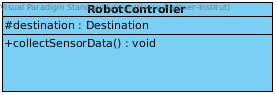
\includegraphics[width=0.6\textwidth]{../images/Iteration0_Entwurf_7-1-1_Klasse_RobotController}
%		\caption{\textcolor{blue}{Durch eigene Diagramme ersetzen}}
%		\label{BeschreibungKlasse1}
%		\end{figure}
		
		%#destination : Destination
		Die Klasse \textit{RobotController} ist die Hauptklasse des \textit{Robots}, 
		da sie den aktuellen Zustand des \textit{Robots} enthält.
		So hat diese Klasse die Möglichkeit, maximal eine \textit{Destination} zu speichern. 
		Diese \textit{Destination} kann ein vom \textit{Server} zugeteiltes Ziel sein, 
		der dem \textit{Robot} zugehörige \textit{Charger}, oder gerade kein Ziel, 
		also \texttt{null} sein. Nur wenn der \textit{Robot} gerade keine \textit{Destination} 
		gespeichert hat, kann er neue Aufträge vom \textit{Server} annehmen.

			%7.1.1.1 #collectSensorData():void
			\paragraph{Beschreibung der Methode \textit{collectSensorData}}
			Der Server kann einen \textit{Robot} dazu auffordern, ihm seine Sensordaten zu schicken. Der \textit{Robot} fragt dann seine Hardwareschnittstelle 
			nach seiner Position und seinem Akkustand an, und gibt diese Informationen, zusammen mit Informationen über den Aktuellen Zustand des \textit{Robots} bzw. seine aktuelle \textit{Destination}, zurück and den \textit{Server}.
	%7.1.2 DrivingSystem
	\subsubsection{Beschreibung der Klasse \textit{DrivingSystem}}
%		\begin{figure}[H]
%		\centering
%		\includegraphics[width=0.6\textwidth]{../images/Iteration0_Entwurf_7-1-2_Klasse_DrivingSystem}
%		\caption{\textcolor{blue}{Durch eigene Diagramme ersetzen}}
%		\label{BeschreibungKlasse1}
%		\end{figure}
		
		%#currentSpeed:float
		Diese Klasse beschreibt den aktuellen Zustand des Fahrsystems des \textit{Robots}. 
		Es sind Informationen über die aktuelle Geschwindigkeit enthalten und die Methode, 
		die gerade ausgeführt wird, gibt Auskunft über die aktuelle Beschäftigung des \textit{Robots}.

			%7.1.2.1 	#driveToDestination(destination: Destination, arrivalHandler: ArrivalHandler): void
			\paragraph{Beschreibung der Methode \texttt{driveToDestination}}
			\begin{figure}[H]
			\centering
			\includegraphics[width=0.9\textwidth]{../images/Iteration0_Entwurf_7-1-2-1_Methode_driveToDestination}
			\caption{Aktivitätsdiagramm zu Metode \texttt{driveToDestination}}
			\label{AktivitaetDriveToDestination}
			\end{figure}

			Wenn diese Methode aufgerufen wird, macht der \textit{Robot} sich auf den Weg zur 
			übergebenen \textit{Destination}. Wenn der \textit{Robot} an dieser \textit{Destination} 
			angekommen ist, wird die \texttt{arrive}-Methode des übergebenen \textit{ArrivalHandlers} ausgeführt. 
			Wenn sich ein \textit{Obstacle} auf dem Weg befindet, wird die Methode \texttt{driveAroundObstacle} 
			aufgerufen, bis das \textit{Obstacle} umfahren wurde.
			
			Abbildung \ref{AktivitaetDriveToDestination} zeigt ein entsprechendes Aktivitätsdiagramm.

			%7.1.2.2    -driveAroundObstacle(destination: Destination): void
			\paragraph{Beschreibung der Methode \texttt{driveAroundObstacle}}
			\begin{figure}[H]
			\centering
			\includegraphics[width=0.7\textwidth]{../images/Iteration0_Entwurf_7-1-2-2_Methode_driveAroundObstacle}
			\caption{Sequenzdiagramm zur Beschreibung der Methode \texttt{driveAroundObstacle}}
			\label{SequenzDriveAroundObstacle}
			\end{figure}

			Diese Methode wird von \texttt{driveToDestination} mit des Position eines \textit{Obstacles} aufgerufen, 
			wenn ein \textit{Obstacle} zu umfahren ist.
			Dabei entscheidet sich der Roboter zunächst ob er links oder rechts an dem \textit{Obstacle} vorbeifährt, 
			und hält sich dann mithilfe seiner Sensoren immer auf einem bestimmten Abstand zum Hindernis, bis zwischen 
			\textit{Obstacle} und der Luftlinie zur \textit{Destination} genug Platz für den \textit{Robot} ist.
			
			Abbildung \ref{SequenzDriveAroundObstacle} zeigt ein entsprechendes Sequenzdiagramm. Dabei ist \texttt{min_dist} eine vorher festgelegte Konstante, welche die Mindestdistanz, die der \textit{Robot} halten muss, wenn er an einem \textit{Obstacle} vorbeifährt, speichert.
	
\pagebreak
	
%7.2 Paket Server
\subsection{Paket \textit{Server}}
%\begin{figure}[H]
%	\centering
%	\includegraphics[width=0.6\textwidth]{../images/Paketdetails.png}
%	\caption{\textcolor{blue}{HIER KOMMT DAS Server - PAKETDIAGRMAM HIN}}
%	\label{Paketdetails}
%	\end{figure}
	Im folgenden beschreiben wir die wichtigen Klassen des Pakets \textit{Server} 
	und ihre zugehörigen Methoden, sowie ihre Interaktion zwischeneinander. 


	%7.2.1 TaskSystem
	\subsubsection{Beschreibung der Klasse \textit{TaskSystem}}
		%	-taskDistribution
		Das \emph{TaskSystem} des \emph{Servers} verarbeitet alle \emph{Tasks}, die es mit der Zuordnung vom \emph{RobotControlSystem} übergeben bekommt. Dafür besitzt es eine Struktur, die die \emph{taskDistribution} intern verwaltet und somit die \emph{Tasks} und die jeweils zugeordneten \emph{Robots} kennt.
		
		%7.2.2.1	~assignTask(virtualRobot : VirtualRobot, destination : Destination): void
			\paragraph{Beschreibung der Methode \texttt{assignTask}}
			Die Methode \texttt{assignTask} führt die Zuordnung und Abspeicherung der Roboter und \emph{Tasks} bzw. \emph{Destinations} durch.
			
	%7.2.2 RobotControlSystem
	\subsubsection{Beschreibung der Klasse \textit{RobotControlSystem}}
		Das \emph{RobotControlSystem} sorgt bei eingehenden \emph{Tasks} dafür, dass ein passender \emph{Robot} ausgewählt wird. Diese Information übergibt es dann an das \emph{TaskSystem}, das für die endgültige Zuordnung zuständig ist.
	
			%7.2.1.1	~chooseRobot(destination: Destination): void
			\paragraph{Beschreibung der Methode \texttt{chooseRobot}}
			Die Methode \texttt{chooseRobot} wählt für den aktuell eingegangenen \emph{Task} einen \emph{Robot} aus. Dazu fragt es die Sensorwerte der verschiedenen \emph{Robotes} ab und wählt den am besten geeigneten aus.
